\documentclass[frame number]{beamer}
\usepackage[utf8]{inputenc}
\usepackage{tikz}
\usetikzlibrary{arrows,decorations,positioning,fit}

\tikzset{%
  post/.style={rectangle,draw=blue!70,top color=white,bottom color=blue!20,very thick},
  user/.style={circle,top color=white,draw=red!70,bottom color=red!20,very thick},
  plain/.style={rectangle,draw=black!70,top color=white, bottom color=black!20,very thick}%
}

\usetheme{Ilmenau}

%% META DATA
\title{Interesting Content and User Discovery without Upvotes}
\subtitle{An application of centrality measures to Reddit}
\author{Rollen S. D'Souza \\ {\texttt{rollen.dsouza@uwaterloo.ca}}}
\institute{University of Waterloo}
\date{2018}

\begin{document}

\frame{\titlepage}

%% OUTLINE
\begin{frame}
  \frametitle{Outline}
  \tableofcontents
\end{frame}

%% INTRODUCTION
\section{Introduction}
\subsection{About Reddit}

\begin{frame}
  \frametitle{What is Reddit?}
  \framesubtitle{Purposes}
  \begin{itemize}
    \item<1->{Social news aggregation}
    \item<2->{Discussion platform}
    \item<3->{Community for help or relaxation}
  \end{itemize}
\end{frame}

\begin{frame}
  \frametitle{What is Reddit?}
  \framesubtitle{Basic Structure}
  \begin{figure}
    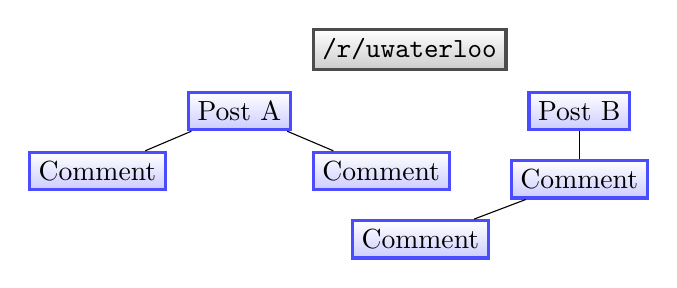
\begin{tikzpicture}[node distance=1em]
      \node (subreddit) [plain] {\texttt{/r/uwaterloo}};
      \node (post_a) [post, below left=of subreddit] {Post A};
      \node (post_b) [post, below right=of subreddit] {Post B};
      \node (comment_1) [post,below left=of post_a] {Comment};
      \node (comment_2) [post,below right=of post_a] {Comment};
      \node (comment_3) [post,below = of post_b] {Comment};
      \node (comment_4) [post,below left=of comment_3] {Comment};

      \path (post_a) edge[-] (comment_1)
            (post_a) edge[-] (comment_2);
      \path (post_b) edge[-] (comment_3) (comment_3) edge[-] (comment_4);

    \end{tikzpicture}
    \caption{Graph-like structure of the Reddit platform.}
    \label{fig:reddit:graph}
  \end{figure}
\end{frame}

\begin{frame}
  \frametitle{What is Reddit?}
  \begin{center}
    
\includegraphics[height=0.85\textheight, keepaspectratio=true]{figures/example_submission}
  \end{center}
\end{frame}

\subsection{Mathematical Preliminaries}
\begin{frame}
  \frametitle{Mathematical Preliminaries}
  What I assume:
  \begin{itemize}
    \item{Centrality Measures}
    \item{Properties of Laplacians}
  \end{itemize}
  The former is how I sort through content and users.
\end{frame}
\begin{frame}
  \frametitle{Katz Centrality Measure}
  \begin{definition}
    The \emph{Katz Centrality Measure} for a node \(i\) in graph \(G\) with adjacency matrix \(A\) is defined as,
    \[
      c_i = \sum_{k=1}^\infty \sum_{j=1}^n \alpha^k \left( A_{j,i} \right)^k,
    \]
    where \(0 < \alpha \leq \rho(A).\)
  \end{definition}
\end{frame}
\begin{frame}
  \frametitle{Katz Centrality Measure}
  \framesubtitle{Why this measure?}
  \begin{itemize}
    \item{Has larger reach in the graph (looks at all paths to a node.)}
    \item{Easy to compute.}
    \item{Loose requirements on \(A.\)}
    \item{Intuitive meaning.}
  \end{itemize}
\end{frame}
\begin{frame}
  \frametitle{On Laplacians}
  Laplacians can be used for clustering. Recall,
  \[
    L = D_{out} - A.
  \]
  Use eigenvalues near 0 for clustering (eigenvectors associated with nearly disconnected components).
  \pause

  So...finding eigenvalues is easy right?
\end{frame}
\begin{frame}
  \frametitle{On Laplacians}
  \framesubtitle{Different Formulation}
  \textbf{Problem:} The graph can have as many as \(10^4\) nodes!
  \pause
  \begin{definition}
    The \emph{normalized Laplacian} of a graph is defined as,
    \[
      L_{rw} = I_{n\times n} - D_{out}^{-1} A
    \]
  \end{definition}
  \pause
  \emph{Need to ensure the graph has no sinks!}
\end{frame}

\section{Analysis}
\subsection{Technical Details}
\begin{frame}
  \frametitle{Technical Details}
  \framesubtitle{The Code}
  Code was implemented using \texttt{Python 3} and \texttt{MATLAB}. Code is available on my Github. Other than that,
  \begin{itemize}
    \item \texttt{redis} for storing data in-memory.
    \item \texttt{numpy},\texttt{scipy} for computation outside of \texttt{MATLAB}.
  \end{itemize}
\end{frame}
\begin{frame}
  \frametitle{Technical Details}
  \framesubtitle{The Data}
  Sourced thanks to Jason Baumgartner who uploaded data dumps of the JSON objects gathered from the Reddit API. Structures contain,
  \begin{itemize}
    \item Submissions with author (id and flair), tags, score, text or link,
    \item Comments with author (id and flair), text
    \item and much much more!
  \end{itemize}
\end{frame}


\end{document}

